\documentclass[12pt]{article}
\usepackage[margin=1in]{geometry}
\usepackage{amsmath, amssymb}
\usepackage{graphicx}
\usepackage{enumitem}
\usepackage{mleftright}
\usepackage{stackengine}
\usepackage{glossaries}
\usepackage{xcolor}
\usepackage{tikz}
\usetikzlibrary{arrows,positioning, shapes.geometric, calc}

\tikzset{
block/.style = {draw, fill=white, rectangle, minimum height=3em, minimum width=3em},
tmp/.style  = {coordinate}, 
sum/.style= {draw, fill=white, circle, node distance=1cm},
input/.style = {coordinate},
output/.style= {coordinate},
pinstyle/.style = {pin edge={to-,thin,black}
}
}

\tikzstyle{process} = [rectangle, rounded corners, minimum width=0.8*1.618cm, minimum height=0.8*1cm,text centered, draw=black]
\tikzstyle{function} = [circle, rounded corners, minimum width=0.5*1.618cm,text centered, draw=black]
\tikzstyle{joint} = [circle, minimum width=0.1cm, draw=black,scale=0.2]
\tikzstyle{point} = [coordinate]
\tikzstyle{nonterminal} = [rectangle, minimum size=12mm, very thick, draw=black, rounded corners, scale=0.75]
\tikzstyle{small} = [rectangle, minimum size=12mm, very thick, draw=black, rounded corners, scale=0.5]

\newtheorem{theorem}{Theorem}[section]
\newtheorem{corollary}{Corollary}[theorem]
\newtheorem{lemma}[theorem]{Lemma}
 

\newacronym{ekf}{EKF}{\textit{Extendted Kalman Filter}}
\newacronym{ckf}{CKF}{\textit{Cubature Kalman Filter}}
\newacronym{ukf}{UKF}{\textit{Unscented Kalman Filter}}
\newacronym{pdf}{PDF}{\textit{Probability Density Function}}
\newacronym{kf}{KF}{\textit{Kalman Filter}}


\def\delequal{\mathrel{\ensurestackMath{\stackon[1pt]{=}{\scriptstyle\Delta}}}}

\newcommand*\diff{\mathop{}\!\mathrm{d}}
\newcommand\at[2]{\left.#1\right|_{#2}}

\begin{document}
%%%%%%%%%%%%%%%%%%%%%%%%%%%%%%%%%%%%%%%%%%%%%%%%%%%%%%%%%%%%%%%%%%%%%%%%%%%
\begin{titlepage}
	\begin{center}
        \textbf{\LARGE{NORTHEASTERN UNIVERSITY}} \\
                \vspace{2mm} %5mm vertical space
            \textbf{\Large{Department of Electrical and Computer Engineering}}\\
                \vspace{15mm} %5mm vertical space
            \LARGE\textsc{2019 PhD Qualifying Examination} \\
                \vspace{2mm} %5mm vertical space
            \Large \textit{in} \\
            \Large\textsc {Communications, Control, and Signal Processing}\\
                \vspace{30mm} %5mm vertical space
            \textbf{\LARGE{Mahdiar Sadeghi}} \\
            \textbf{\LARGE{Problem 4}} \\
            \textbf{\LARGE{03/11/2019}}

    \end{center}
\end{titlepage}
%%%%%%%%%%%%%%%%%%%%%%%%%%%%%%%%%%%%%%%%%%%%%%%%%%%%%%%%%%%%%%%%%%%%%%%%%%%
\section*{Problem 4: Nonlinear Dynamic State Estimation}

All solutions in this report are based on a time-invariant nonlinear state space model of the form \eqref{eq:def}. The $f(.)$ and $h(.)$ are multivariate functions of the state space $x_k$, and additive noises $\{w_k\}$, $\{\nu_k\}$ are i.i.d processes independent of each other of the initial state $x_0$.  Fig.~\ref{fig:model} is an illustration of this model.  
    %
    \begin{align} \label{eq:def}
        \begin{split}
            x_{k+1} &= f(x_{k}) + w_{k}, \\
            y_k &= h(x_k) + v_k.
        \end{split}
        \qquad \qquad \qquad 0 \leq k
    \end{align}
    %
%
\begin{figure}[!ht] \centering
    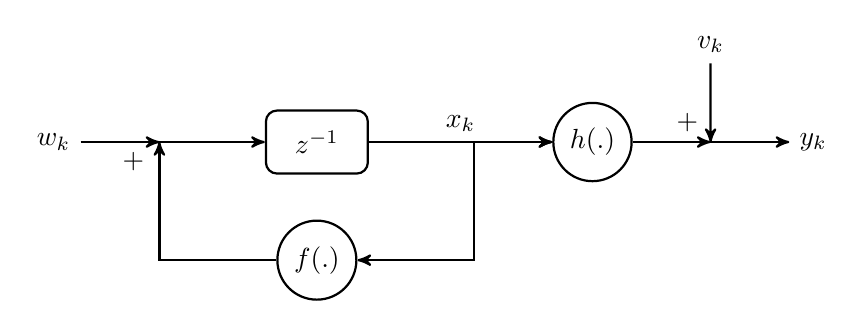
\begin{tikzpicture}[auto, scale=1, node distance=1.5cm,>=latex', point/.style={coordinate},>=stealth',thick] 
            \node (z-1) [process] {$z^{-1}$};
            \node (A) [function, below of=z-1] {$f(.)$};
            \node (C) [function, right of=z-1, xshift=2cm] {$h(.)$};
            \node (sum2)[point, right of=z-1, xshift=0.5cm] {};
            \node (sum1)[point, left of=z-1, xshift=-0.5cm]  {};
            \node (sum3)[point, right of=C]  {};

            \draw [->] ($(-3cm,0)$)node[left]{$w_{k}$} -- (sum1);
            \draw [<-] ($(6cm,0)$)node[right]{$y_k$} -- (C);
            \draw [->] ($(5cm,1cm)$)node[above]{$v_k$} -- (sum3);
            \draw [->] (z-1)-- node{$x_k$}(C);
            \draw [->] (C)--node[above, xshift=0.2cm]{$+$}(sum3);
            \draw [->] (sum1)--node[below, xshift=-1cm]{$+$}(z-1);
            \draw [->] (sum2)--(C);
            \draw [->] (sum2)|-(A);
            \draw [->] (A)-|(sum1);
            \end{tikzpicture}
        \caption{Block diagram of the nonlinear state space model \eqref{eq:def}. } \label{fig:model}
    \end{figure}

%%%%%%%%%%%%%%%%%%%%%%%%%%%%%%%%%%%%%%%%%%%%%%%%%%%%%%%%%%%%%%%%%%%%%%%%%%%
\subsection*{Part A}
    Discussion of the \acrfull{ekf}.
    
\begin{enumerate}[label=\arabic*)]

    \item 
        The linearized version of the nonlinear state-space model \eqref{eq:def} subject to \acrshort{ekf} is obtained by a first order Taylor expansion:
        %
        \begin{align} \label{eq:lin}
            \begin{split}
                x_{k+1} &= f(\hat x_{k|k}) + F(\hat x_{k|k}) (x_k - \hat x_{k|k}) + w_k, \\
                y_k &= h(\hat x_{k|k-1}) + H(\hat x_{k|k-1}) (x_k - \hat x_{k|k-1}) + v_k.
            \end{split}
        \end{align}
        %
        The $F(\hat x_{k|k})\delequal\at{\frac{\partial f}{\partial x}}{x=\hat x_{k|k}}$ and $H(\hat x_{k|k-1}) \delequal \at{\frac{\partial h}{\partial x}}{x=\hat x_{k|k-1}}$ are Jacobian matrices. Both matrices are (i) time-invariant, and (ii) stochastic. \acrshort{ekf} does not take into account that $x_k$ is a random variable with inherent uncertainty, and this is true when the first two terms of the Taylor series are dominating the remaining terms. 
        
    \item
        The idea of \acrshort{ekf} is to assume quasi-linear behavior for a nonlinear system. Assuming that the process noise $w_k$ and the measurement noise $v_k$ are zero mean with covariance $W_k$ and $V_k$, and the initial state is $x_0$. The time-update~\eqref{eq:ekf_t} and measurement-update~\eqref{eq:ekf_m} are the corresponding \acrshort{ekf} explicit recursions \cite{gustafsson2010particle, sarkka2013bayesian} to the model~\eqref{eq:lin}.
        %
        \begin{subequations}  \label{eq:ekf_t}
        \begin{align} 
            \hat x_{k+1|k} &= f(\hat x_{k|k}), 
            \label{eq:ekf_t1} \\
            P_{k+1|k} &= F(\hat x_{k|k}) P_{k|k} F^T(\hat x_{k|k}) + W_k.
            \label{eq:ekf_t2} 
        \end{align} 
        \end{subequations}
        %
        \begin{subequations}    \label{eq:ekf_m}
        \begin{align}
            P_{yy, k|k-1} &= H(\hat x_{k|k-1}) P_{k|k-1} H^T(\hat x_{k|k-1}) + V_k, \label{eq:ekf_m1}\\
            P_{xy, k|k-1} &= P_{k|k-1} H^T(\hat x_{k|k-1}), \label{eq:ekf_m2}\\
            K_k &= P_{xy,k|k-1} P^{-1}_{yy,k|k-1}, \label{eq:ekf_m3} \\
            \hat x_{k|k} &= \hat x_{k|k-1} + K_k (y_k - h(\hat{x}_{k|k-1})), \label{eq:ekf_m4}\\
            P_{k|k} &= P_{k|k-1} - K_k P_{yy,k|k-1} K_k^T. \label{eq:ekf_m5} 
        \end{align}
        \end{subequations}
        %
        
        %
        Higher order \acrshort{ekf} is defined based on second order Taylor expansion using Jacobian and Hessian matrices. \acrshort{ekf} analysis here are based on \eqref{eq:ekf_t} and \eqref{eq:ekf_m}.
        
    \item
    
        Block diagram of \acrshort{ekf} is represented in Fig. \ref{fig:ekf}. The dashed blue rectangular is the time-update module. It takes the process noise variance $W_k$, the mean $\hat{x}_{k-1|k-1}$ and covariance $P_{k-1|k-1}$ of the previous estimation, then calculates predicts the mean $\hat{x}_{k|k-1}$ and covariance $P_{k|k-1}$ of the next state using Eq.~\eqref{eq:ekf_t}.  The dashed red rectangular is the measurement-update module. It takes the output of time-step along with the new measurement $y_k$, and the measurement noise variance $V_k$, then calculates the mean $\hat{x}_{k|k}$ and covariance $P_{k|k}$ of the next system state using Eq.~\eqref{eq:ekf_m}.  
    
        \begin{figure}[!ht] \centering
        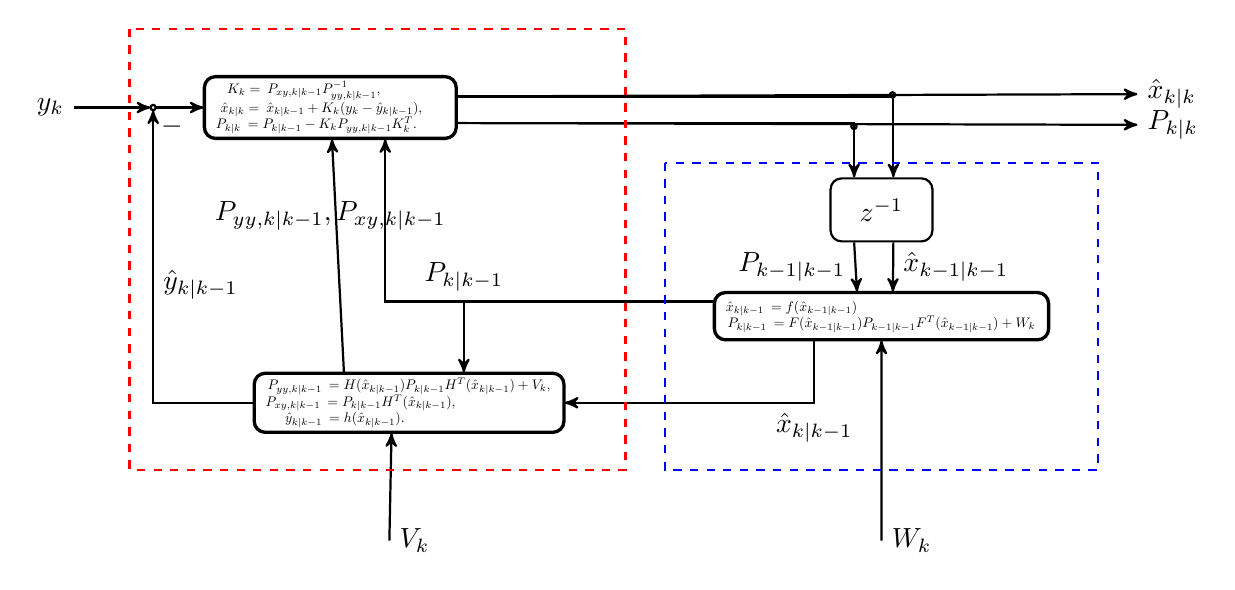
\begin{tikzpicture}[auto, node distance=1.5cm,>=latex',>=stealth',thick]
            \node (sum1) [joint] {};
            \draw [->] ($(-1cm,0)$)node[left]{$y_k$} -- (sum1);
            \node (K)  [small, right of=sum1, xshift=3cm] {$\begin{array}{cc} 
            K_k =\: P_{xy,k|k-1} P^{-1}_{yy,k|k-1}, \quad  \qquad \; \; \; \\
            \hat x_{k|k} =\: \hat x_{k|k-1} + K_k (y_k - \hat{y}_{k|k-1}), \quad \; \\
            P_{k|k} \:= P_{k|k-1} - K_k P_{yy, k|k-1} K_k^T. \qquad \end{array}$}; 
            \node (id2)  [small, below of=K, yshift=-6cm, xshift=2cm] {$\begin{array}{cc} 
            P_{yy, k|k-1} \:= H(\hat x_{k|k-1}) P_{k|k-1} H^T(\hat x_{k|k-1}) + V_k, \\
            P_{xy, k|k-1} \:= P_{k|k-1} H^T(\hat x_{k|k-1}), \qquad \qquad \qquad \quad \\
            \hat{y}_{k|k-1} \:= h(\hat x_{k|k-1}).  \qquad \qquad \qquad \qquad \quad \;  \end{array}$}; 
            \node (delay) [process, below of=K, xshift=7cm, yshift=.2cm] {$z^{-1}$};
            \node (1) [joint, above of=delay, xshift=0.7cm, yshift=5.8cm] {};
            \node (2) [joint, above of=delay, xshift=-1.75cm, yshift=3.8cm] {};
            \node (T)  [small, below of=delay, yshift=-1.2cm] {$\begin{array}{cc} 
            \hat{x}_{k|k-1} \:= f(\hat x_{k-1|k-1}) \qquad \qquad \qquad \qquad \qquad \qquad \quad\\
            P_{k|k-1} \:= F(\hat x_{k-1|k-1}) P_{k-1|k-1} F^T(\hat x_{k-1|k-1}) + W_k\end{array}$}; 
            \draw [->] (K.5) --($(12.5cm,.17cm)$)node[right]{$\hat{x}_{k|k}$} ;
            \draw [->] (K.-7) --($(12.5cm,-.22cm)$)node[right]{$P_{k|k}$} ;
            \draw [<-] (T.-90) --($(9.25cm,-5.5cm)$)node[right]{$W_k$} ;
            \draw [<-] (id2.-120) --($(3cm,-5.5cm)$)node[right]{$V_k$} ;
            \draw [->] (K.5) -| (delay.70);
            \draw [->] (K.-7) -| (delay.130);
            \draw [->] (id2.155) -- node[left, yshift=.5cm, xshift=1.5cm]{$P_{yy,k|k-1}, P_{xy,k|k-1}$}(K);
            \draw [->] (id2) -| node[right, yshift=1.5cm]{$\hat{y}_{k|k-1}$}(sum1);
            \draw [->] (sum1) -- node[below, xshift=-.1cm] {$-$}(K);
            \draw [->] (delay.-70) -- node[right]{$\hat{x}_{k-1|k-1}$}(T.65);
            \draw [->] (delay.-130) -- node[left]{$P_{k-1|k-1}$}(T.135);
            \draw [->] (T.175) -| node[above,xshift=1cm]{$P_{k|k-1}$}(K.-30);
            \draw [->] (T.175) -| (id2.29);
            \draw [->] (T.-160) |- node[below]{$\hat{x}_{k|k-1}$}(id2);
            \draw[red,thick,dashed] (-.3,1)  rectangle (6,-4.6);
            \draw[blue,thick,dashed] (6.5,-.7)  rectangle (12,-4.6);
            \end{tikzpicture}
            \caption{\acrshort{ekf} block diagram. Time-update and measurement-update blocks are represented by blue and red dashed rectangular.} \label{fig:ekf}
        \end{figure}
        
        The measurement variable directly influences the estimated state mean $\hat{x}_{k|k}$ and maximum covariance $P_{k|k}$, therefore all variables are dependent of the measurement recursively, except the measurement noise $v_k$ and process noise $w_k$.
        
        The system will be independent of measurement in case of high measurement noise covariance $V_k$. In this case Kalman gain $K_k$ goes to zero, and the estimated state will depend on predicted state $\hat{x}_{k|k}$ only. It is obvious that a measurement with high uncertainty is not valuable and \acrshort{kf} reduces the weight of the measured (observed) value in consequence.
        
        
    \item
        Kalman's original derivation did not apply Bayes' rule and does not require the exploitation of any specific error distribution information beyond the mean and covariance \cite{kalman1960new}. However, the filter yields the exact conditional probability estimate in the special case that all errors are Gaussian. \acrshort{kf} can be derived as an application of Bayes' rule under the assumption that all estimates have independent, Gaussian distributed errors \cite{julier2004unscented}. 
        
        
    \item
        The innovation process can be rewritten as $y_k - \hat{y}_{k|k-1}$. It is the difference between the actual measurement $y_k$ and its estimated prediction, based on the system model and previous measurement $\hat{y}_{k|k-1}$.
        %
        The first two moments of the innovation signal is known. The mean is zero. The covariance matrix of innovation based on the linearized model is given by \eqref{eq:ekf_m1}.
        If the noise assumed to be Gaussian, then the innovation sequence is zero-mean, white (uncorrelated), with covariance equal to the measurement prediction covariance, and has a Gaussian distribution. 
\end{enumerate}
%%%%%%%%%%%%%%%%%%%%%%%%%%%%%%%%%%%%%%%%%%%%%%%%%%%%%%%%%%%%%%%%%%%%%%%%%%%
\subsection*{Part B}
    Discussion of the \acrfull{ckf}.
    
\begin{enumerate}[label=\arabic*)]

    \item
        \textit{Bayesian filtering} aims to compute the posterior density $p(x_k|y_{1:k})$ of the state $x_k$ at each time step $k$, given the history of the measurement up to the time step $k$ and the prior density $p(x_{k-1}|y_{1:k-1})$ \cite{sarkka2013bayesian}. The recursions start from the initial distribution $p(x_0)$, then applying two step recursive algorithm: times-update~\eqref{eq:bf_t} which is derived by \textit{Chapman-Kolmogorov equation}, and measurement-step~\eqref{eq:bf_m} which is derived by \textit{Bayes' rule}. 
        %
        \begin{align} \label{eq:bf_t}
            p(x_k|y_{1:k-1}) &= \int p (x_k|x_{k-1}) p(x_{k-1}|y_{1:k-1}) \diff{x_{k-1}} 
        \end{align}
        \begin{subequations} \label{eq:bf_m}
        \begin{align}
            p(x_k|y_{1:k}) &= \frac{1}{c_k} p (y_k|x_k) p(x_k|y_{1:k-1}) \label{eq:bf2} \\
            c_k &= \int p (y_k|x_k) p(x_k|y_{1:k-1}) \diff{x_k} \label{eq:bf3}
        \end{align}
        \end{subequations}
        %
        The integrals of Eq.~\eqref{eq:bf_t} and \eqref{eq:bf3} need to be computed in the general Bayesian filtering. However, from practical perspective they are intractable \cite{arasaratnam2009cubature}. Notable exceptions in which optimal solution is tractable are including: Linear-Gaussian dynamic system (\acrshort{kf} \cite{kalman1960new}), discrete-valued state-space with a fixed number of states (Hidden-Markov model filter \cite{liu2008monte}), and \textit{Benes type} of non-linearity \cite{benevs1981exact}. 
    \item 
        For the case of Gaussian state-spaces, the predictive \acrshort{pdf} $p(x_k|y_{1:k-1})$ and the filter likelihood \acrshort{pdf} $p(x_k|y_{1:k})$ are both assumed to be Gaussian.
        In the time-update step, the $p(x_k|y_{1:k-1})$ is $\mathcal{N}(\hat x_{k|k-1},P_{k|k-1})$. Where the mean and covariance are defined by the statistical expectation operator $\mathbb E[.]$ as following.
        %
        \begin{subequations}\label{eq:bfg_t}
        \begin{align}
            \hat x_{k|k-1} &= \mathbb E[x_k|y_{1:k-1}] = \mathbb E[f(x_{k-1}) + w_k|y_{1:k-1}] \label{eq:bfg_t1}\\
            &= \mathbb E[f(x_{k-1}) |y_{1:k-1}] \label{eq:bfg_t2}\\
            &= \int f(x_{k-1}) p(x_{k-1}|y_{1:k-1}) \diff{x_{k-1}} \label{eq:bfg_t3}\\
            &= \int f(x_{k-1}) \times \mathcal{N} (x_{k-1}|\hat x_{k-1|k-1}, P_{k-1|k-1}) \diff{x_{k-1}} \label{eq:int_1}
        \end{align}
        \end{subequations}
        %
        It is possible to write \eqref{eq:bfg_t1} from \eqref{eq:bfg_t2} by assuming that the process noise $w_k\sim\mathcal{N}(0,W_k)$ is zero-mean and uncorrelated with the past measurements.
        %
        \begin{subequations}\label{eq:bfg_m}
        \begin{align}
            P_{k|k-1} &= \mathbb E[(x_k-\hat x_{k|k-1})(x_k-\hat x_{k|k-1})^T|y_{1:k-1}] \label{eq:bfg_m1}\\
            &= \mathbb E[(f(x_{k-1})+w_{k-1}-\hat x_{k|k-1})(f(x_{k-1})+w_{k-1}-\hat x_{k|k-1})^T|y_{1:k-1}] \label{eq:bfg_m2} \\
            \begin{split}
            &= \mathbb E[ f(x_{k-1})f^T(x_{k-1}) + f(x_{k-1})  w^T_{k-1} - f(x_{k-1}) \hat x^T_{k|k-1} \\ 
            & \qquad \qquad + w_{k-1} f^T(x_{k-1}) + w_{k-1} w^T_{k-1} - w_{k-1} \hat x^T_{k|k-1} \\ 
            & \qquad \qquad \qquad \qquad - \hat x_{k|k-1} f^T(x_{k-1}) - \hat x_{k|k-1}  w^T_{k-1} + \hat x_{k|k-1}  \hat x^T_{k|k-1} |y_{1:k-1}] 
            \end{split}
            \label{eq:bfg_m3} \\
            \begin{split}
            &= \int f(x_{k-1})f^T(x_{k-1}) \times \mathcal{N} (x_{k-1}|\hat x_{k-1|k-1}, P_{k-1|k-1}) \diff{x_{k-1}} \\
             & \qquad \qquad \qquad -\hat x_{k-1|k-1} \hat x^T_{k-1|k-1} + W_{k-1} 
            \end{split} \label{eq:int_2}
        \end{align}
        \end{subequations}
        %
        
        %
        In the measurement-update step, the $p(y_k|y_{1:k-1})$ is $\mathcal{N}(\hat y_{k|k-1},P_{yy,k|k-1})$.
        %
        \begin{subequations}\label{eq:bfg_my}
        \begin{align}
            \hat y_{k|k-1} &= \mathbb E[y_k|y_{1:k-1}] = \mathbb E[h(x_{k}) + v_k|y_{1:k-1}] \label{eq:bfg_my1} \\
            &= \mathbb E[h(x_{k})|y_{1:k-1}] \label{eq:bfg_my2} \\
            &= \int h(x_{k}) \times \mathcal{N} (x_{k}|\hat x_{k|k-1}, P_{k|k-1}) \diff{x_{k}} \label{eq:int_3}
        \end{align}
        \end{subequations}
        %
        %
        \begin{subequations}\label{eq:bfg_myp}
        \begin{align}
            P_{yy,k|k-1} &= \mathbb E[y_k-\hat y_{k|k-1})(y_k-\hat y_{k|k-1})^T|y_{1:k-1}]  \label{eq:bfg_myp1} \\
            &= \mathbb E[(h(x_k)+v_k-\hat y_{k|k-1})(h(x_k)+v_k-\hat y_{k|k-1})^T|y_{1:k-1}]  \label{eq:bfg_myp2} \\
            &= \int h(x_{k})h^T(x_{k}) \times \mathcal{N} (x_{k}|\hat x_{k|k-1}, P_{k|k-1}) \diff{x_{k}} - \hat y_{k|k-1} \hat y^T_{k|k-1} + V_{k}  \label{eq:int_4}
        \end{align}
        \end{subequations}
        %
        \begin{subequations}\label{eq:bfg_myz}
        \begin{align}
            P_{xy,k|k-1} &= \mathbb E[(x_k-\hat x_{k|k-1})(y_k-\hat y_{k|k-1})^T|y_{1:k-1}]  \label{eq:bfg_myz1} \\
            &= \mathbb E[(x_k-\hat x_{k|k-1})(h(x_k)+v_k-\hat y_{k|k-1})^T|y_{1:k-1}]  \label{eq:bfg_myz2} \\
            \begin{split}
            &= \mathbb E[ x_k h^T(x_k) + x_k v^T_k - x_k \hat y^T_{k|k-1} 
            - \hat x_{k|k-1} h^T(x_k) \\
            & \qquad \qquad \qquad  \qquad \qquad - \hat x_{k|k-1} v^T_k + \hat x_{k|k-1} \hat y^T_{k|k-1} | y_{1:k-1}] 
            \end{split}
            \label{eq:bfg_myz3} \\
            &= \int x_k h^T(x_{k}) \times \mathcal{N} (x_{k}|\hat x_{k|k-1}, P_{k|k-1}) \diff{x_{k}} - \hat x_{k|k-1} \hat y^T_{k|k-1}   \label{eq:int_5}
        \end{align}
        \end{subequations}
        %
        Therefore, the conditional Gaussian density of the joint state and the measurement is:
        \begin{align} \label{eq:cond}
            p \left( \left[ \left. {\begin{array}{c}
                x_k \\
                y_k \\
            \end{array} } \right] \right| y_{1:k-1}  \right) =
            \mathcal{N} \left( \left( {\begin{array}{c}
                \hat x_{k|k-1} \\
                \hat y_{k|k-1} \\
            \end{array} } \right), 
            \left( {\begin{array}{cc}
                P_{k|k-1} & P_{xy,k|k-1} \\
                P^T_{xy,k|k-1} & P_{yy,k|k-1} \\
            \end{array} } \right) \right)
        \end{align}
        %
        So, the Bayesian filter computes the posterior density $p(x_k|y_k)$ from Eq.~\eqref{eq:cond} as:
        %
        \begin{equation} \label{eq:meas}
            p(x_k|y_k) = \mathcal{N} (x_k|\hat x_{k|k}, P_{k|k})
        \end{equation}
        %
        Upon receiving the new measurement $y_k$, the \acrshort{kf} equations will be used to find the posterior density mean $\hat{x}_{k|k}$ and convariance $P_{k|k}$:
        %
        \begin{subequations} \label{eq:kf}
        \begin{align}
            \hat x_{k|k} &= \hat x_{k|k-1} + K_k (y_k - \hat y_{k|k-1}), \\
            P_{k|k} &= P_{k|k-1} - K_k P_{yy,k|k-1} K_k^T, \\
            K_k &= P_{xy,k|k-1} P^{-1}_{yy,k|k-1}.
        \end{align}
        \end{subequations}
        %
        The main challenge and the heart of the Bayesian filter is to compute Gaussian weighted integrals of \eqref{eq:int_1}, \eqref{eq:int_2}, \eqref{eq:int_3}, \eqref{eq:int_4}, and \eqref{eq:int_5}. They are all in a combination of non-linear function and a Gaussian \acrshort{pdf}. It is not easy to derive this integral analytically for general non-linear state space model, for a linear state space model:
        %
        \begin{subequations}
        \begin{align}
            x_{k+1} &= F_k x_k + w_k, \\
            y_k &= H_k x_k + v_k.
        \end{align}
        \end{subequations}
        %
        The time-update step derivations can be rewritten as:
        %
        \begin{align} \label{eq:linG1}
        \begin{split}
            \hat x_{k|k-1} &= \mathbb E[ F_{k-1} x_{k-1} + w_{k-1} |y_{1:k-1}] = F_{k-1} \mathbb E[ x_{k-1} |y_{1:k-1}] \\
            &= F_{k-1} \hat x_{k-1|k-1}
        \end{split}
        \end{align}
        %
        \begin{align} \label{eq:linG2}
        \begin{split}
            P_{k|k-1} &=  \mathbb E[(x_k-\hat x_{k|k-1})(x_k-\hat x_{k|k-1})^T|y_{1:k-1}] \\
            &= \mathbb E[ ( F_{k-1} x_{k-1} + w_{k-1}- F_{k-1} \hat x_{k-1|k-1})( F_{k-1} x_{k-1} + w_{k-1}- F_{k-1} \hat x_{k-1|k-1})^T|y_{1:k-1}] \\
            &= \mathbb E[ ( F_{k-1} x_{k-1} ) ( F_{k-1} x_{k-1} )^T + ( F_{k-1} x_{k-1} ) w^T_{k-1} - ( F_{k-1} x_{k-1} ) ( F_{k-1} \hat x_{k-1} )^T \\
            & \qquad  + w_{k-1} ( F_{k-1} x_{k-1} )^T + w_{k-1} w^T_{k-1} - w_{k-1} ( F_{k-1} \hat x_{k-1|k-1} )^T  \\ & \qquad \qquad + ( F_{k-1} \hat x_{k-1|k-1} ) (F_{k-1} x_{k-1})^T 
            + ( F_{k-1} \hat x_{k-1|k-1} ) w^T_{k-1} \\ & \qquad \qquad \qquad- ( F_{k-1} \hat x_{k-1|k-1} ) ( F_{k-1} \hat x_{k-1|k-1} )^T|y_{1:k-1}] \\
            &= \mathbb E[ ( F_{k-1} x_{k-1} - F_{k-1} \hat x_{k-1|k-1} ) ( F_{k-1} x_{k-1} - F_{k-1} \hat x_{k-1|k-1} )^T + w_{k-1} w^T_{k-1}|y_{1:k-1}] \\
            &= F_{k-1} \mathbb E[(x_{k-1}-\hat x_{k-1|k-1})(x_{k-1}-\hat x_{k-1|k-1})^T |y_{1:k-1}] F^T_{k-1} + \mathbb E[w_{k-1} w^T_{k-1} |y_{1:k-1}] \\
            &= F_{k-1} P_{k-1|k-1} F^T_{k-1} + W_{k-1}
        \end{split}
        \end{align}
        %
        \begin{align} \label{eq:linG3}
        \begin{split}
            \hat y_{k|k-1} &=  \mathbb E[ H_{k} x_{k} + v_{k} |y_{1:k-1}] = H_{k} \mathbb E[ x_{k} |y_{1:k-1}] \\
            &= H_{k} \hat x_{k|k-1}
        \end{split}
        \end{align}
        %
        And similar to derivation of \eqref{eq:linG2}, the measurement-update step can be rewritten as:
        %
        \begin{align} \label{eq:linG4}
        \begin{split}
            \hat P_{yy,k|k-1} &=  \mathbb E[(y_k-\hat y_{k|k-1})(y_k-\hat y_{k|k-1})^T|y_{1:k-1}] \\
            &= \mathbb E[ ( H_{k} x_{k} + v_{k}- H_{k} \hat x_{k|k-1})( H_{k} x_{k} + v_{k}- H_{k} \hat x_{k|k-1})^T|y_{1:k-1}] \\
            &= H_{k} P_{k|k-1} H^T_{k} + V_{k}
        \end{split}
        \end{align}
        %
        \begin{align} \label{eq:linG5}
        \begin{split}
            \hat P_{xy,k|k-1} &= \mathbb E[(x_k-\hat x_{k|k-1})(y_k-\hat y_{k|k-1})^T|y_{1:k-1}]  \\
            &=  \mathbb E[(x_k-\hat x_{k|k-1})( H_{k} x_{k} + v_{k}- H_{k} \hat x_{k|k-1})^T |y_{1:k-1}]   \\
            &=  \mathbb E[(x_k-\hat x_{k|k-1})( H_{k} x_{k} - H_{k} \hat x_{k|k-1})^T |y_{1:k-1}]  \\
            &= \mathbb E[(x_k-\hat x_{k|k-1})( x_{k} - \hat x_{k|k-1})^T |y_{1:k-1}] H^T_{k}  \\
            &= P_{k|k-1} H^T_{k} 
        \end{split}
        \end{align}
        %
        Now that the predicted density \eqref{eq:cond} is derived for linear state space. The \acrshort{kf} equations are proven to be the same as the conditional distribution of Gaussian variables $x_k$ and $y_k$ for linear Gaussian systems \cite{sarkka2013bayesian}.
        
        \begin{lemma} \label{lem:1}
        If the random variables $x$ and $y$ have the joint Gaussian probability distribution:
        %
        \begin{align} \label{eq:jgp}
            \left(  \begin{array}{c}
                x \\
                y \\
            \end{array}  \right) 
            \sim\mathcal{N} \left( \left( {\begin{array}{c}
                 a \\
                 b \\
            \end{array} } \right), 
            \left( {\begin{array}{cc}
                A & C \\
                C^T & B \\
            \end{array} } \right) \right)
        \end{align}
        %
        The marginal distribution of $x$ and $y$ are given as:
        %
        \begin{subequations} \label{eq:marg}
        \begin{align} 
            x &\sim \mathcal{N}(a, A), \\
            y &\sim \mathcal{N}(b, B), \\
            x|y  &\sim \mathcal{N}(a+CB^{-1}(y-b),A-CB^{-1}C^T), \\
            y|x  &\sim \mathcal{N}(b+C^TA^{-1}(x-a),B-C^TA^{-1}C).
        \end{align}
        \end{subequations}
        % 
        \end{lemma}
        
        The marginal distribution ~\eqref{eq:marg} is proven in Ch. 2 of \cite{bishop2006pattern}. Now, the idea is to write probability density function of variable $x$ from Eq.~\eqref{eq:jgp} and consider $y$ as a constant variable to find mean and covariance of $p(x|y)$.
        %
        
        %
        Using the \eqref{eq:linG1}, \eqref{eq:linG2}, \eqref{eq:linG3}, \eqref{eq:linG4}, and \eqref{eq:linG5} as the joint Gaussian \acrshort{pdf} of \eqref{eq:cond}, gives $a=\hat x_{k|k-1}$, $b=\hat y_{k|k-1}$, $A=P_{k|k-1}$, $B=P_{yy,k|k-1}$, and $C=P_{xy,k|k-1}$. The marginal distribution formula \eqref{eq:marg} gives the \acrshort{kf} equations:
        %
        \begin{subequations} \label{eq:kmf}
        \begin{align}
            x_k & \sim \mathcal{N} (\hat x_{k|k}, P_{k|k}). \\ 
            \begin{split}
            \hat x_{k|k} &= \hat x_{k|k-1} + P_{xy,k|k-1} P^{-1}_{yy,k|k-1} [y_k - \hat y_{k|k-1}], \\
            &= \hat x_{k|k-1} + K_k [y_k - \hat y_{k|k-1}].
            \end{split} \\
            \begin{split}
            P_{k|k} &= P_{k|k-1} - P_{xy,k|k-1} P^{-1}_{yy,k|k-1} P^T_{xy,k|k-1}, \\
            &= P_{k|k-1} - K_k  P_{yy,k|k-1} K_k^T.
            \end{split} 
        \end{align}
        \end{subequations} 
        %
        Where \eqref{eq:kmf} is rewritten in the form of standard measurement-update \acrshort{kf}  \eqref{eq:ekf_m} by defining Kalman gain as $K_kP_{xy,k|k-1} P^{-1}_{yy,k|k-1}$. The $\hat x_{k|k-1}$ and $P_{k|k-1}$ are the predicted variables from the time-update step \eqref{eq:linG1} and \eqref{eq:linG2}.
        
    \item
        Fig. \ref{fig:ckf} is the block diagram of \acrshort{ckf}. Similar to the \acrshort{ekf} block diagram, the filter is taking the previous state estimate mean $\hat{x}_{k-1|k-1}$ and covariance $P_{k-1|k-1}$ to calculate the new estimate state mean $x_{k|k}$ and covariance $P_{k|k}$.
        
        In the time-update state (illustrated with dashed blue rectangular), the sigma-points $\xi^{(i)}$ are derived based on spherical-radial cubature rules \cite{arasaratnam2009cubature}. Then the sigma points will propagate in the system $f(.)$,  and used for calculation of mean $\hat{x_{k|k-1}}$ and covariance $P_{k|k-1}$ of the predicted state $x_{k|k-1}$.
        
        In the measurement-update state (illustrated with dashed red rectangular), the propagated sigma-points $\xi^{(i)}$ are taken to derive the new sampling points using the square root matrix $S_{k|k-1}$. The propagated sigma-points in the system $h(.)$ will be used for calculation of the mean $\hat{y}_{k|k-1}$, covariance $P_{yy,k|k-1}$, and cross covariance $P_{xy,k|k-1}$. On the top left of the Fig. \ref{fig:ckf}, the \acrshort{kf} block takes the new measurement, with the first two moments of predicted measurement and it cross covariance with the predicted state to calculate the best state estimate of the mean $\hat{x}_{k|k}$ and covariance $P_{k|k}$ using represented analytic formulas of standard \acrshort{kf}. 

    \begin{figure}[!ht] \centering
        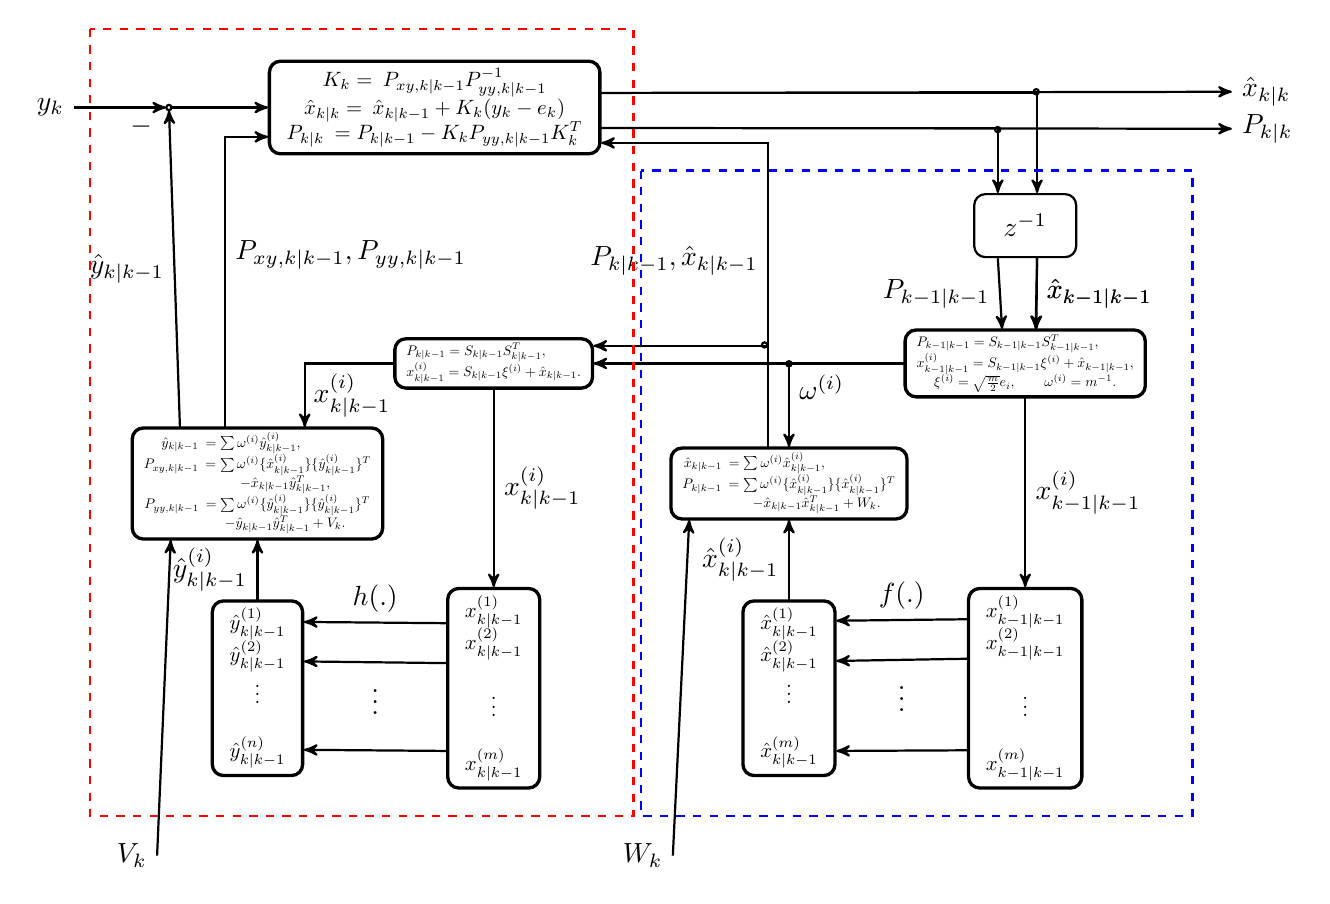
\begin{tikzpicture}[auto, node distance=1.5cm,>=latex',>=stealth',thick]
            \node (sum1) [joint] {};
            \draw [->] ($(-1.2cm,0)$)node[left]{$y_k$} -- (sum1);
            \node (K)  [nonterminal, right of=sum1, xshift=3cm] {$\begin{array}{cc} 
            K_k =\: P_{xy,k|k-1} P_{yy,k|k-1}^{-1}\\
            \hat x_{k|k} =\: \hat x_{k|k-1} + K_k (y_k - e_k) \\
            P_{k|k} \:= P_{k|k-1} - K_k P_{yy,k|k-1} K_k^T \end{array}$}; 
            
            \node (delay) [process, below of=K, xshift=7.5cm] {$z^{-1}$};
            \node (1) [joint, above of=delay, xshift=0.7cm, yshift=7cm] {};
            \node (2) [joint, above of=delay, xshift=-1.75cm, yshift=4.6cm] {};
            
            \node (T)  [small, below of=delay, yshift=-2cm] {$\begin{array}{cc} 
            P_{k-1|k-1} = S_{k-1|k-1} S^T_{k-1|k-1}, \qquad \;\; \\
            x^{(i)}_{k-1|k-1} = S_{k-1|k-1} \xi^{(i)} + \hat{x}_{k-1|k-1}, \\
            \xi^{(i)} = \sqrt{\frac{m}{2}}e_i, \qquad  \omega^{(i)} = m^{-1}. \end{array}$}; 
            
            \node (T2)  [small, left of=T, xshift=-12cm] {$\begin{array}{cc} 
            P_{k|k-1} = S_{k|k-1} S^T_{k|k-1}, \qquad \;\; \\
            x^{(i)}_{k|k-1} = S_{k|k-1} \xi^{(i)} + \hat{x}_{k|k-1}. \end{array}$}; 
            
            \node (S1)  [nonterminal, below of=T, yshift=-4cm] {$\begin{array}{c} 
            x^{(1)}_{k-1|k-1} \\
            x^{(2)}_{k-1|k-1}\\ \\
            \vdots \\ \\
            x^{(m)}_{k-1|k-1} \end{array}$}; 
            
            \node (S2)  [nonterminal, left of=S1, xshift=-2.5cm] {$\begin{array}{c} 
            \hat{x}^{(1)}_{k|k-1} \\ 
            \hat{x}^{(2)}_{k|k-1}\\
            \vdots \\ \\
            \hat{x}^{(m)}_{k|k-1} \end{array}$};
            
            \draw [->] (T) -- node[right]{$x^{(i)}_{k-1|k-1}$}  (S1);
            
            \draw [->] (S1.130) -- node[above]{$f(.)$}(S2.55);
            \draw [->] (S1.153) -- node[below]{$\vdots$}(S2.30);
            \draw [->] (S1.227) -- (S2.-53);
            
            \node (P1) [small , above of=S2, yshift=3.7cm] {$\begin{array}{cc} 
            \hat{x}_{k|k-1} \:= \sum \omega^{(i)} \hat{x}^{(i)}_{k|k-1}, 
            \qquad \qquad \quad \\
            P_{k|k-1} \:= \sum \omega^{(i)} \{ \hat{x}^{(i)}_{k|k-1} \} \{ \hat{x}^{(i)}_{k|k-1} \}^T\\
            \qquad \qquad - \hat{x}_{k|k-1} \hat{x}^T_{k|k-1} + W_k.\end{array}$};
            
            \draw [->] (S2) --  node[left]{$\hat{x}^{(i)}_{k|k-1}$} (P1);
            \draw [->] (T) -| node[right, yshift=-.3cm]{$\omega^{(i)}$} (P1);
            \draw [->] (T) -- (T2);
            
            \node (S3)  [nonterminal, below of=T2, yshift=-4cm] {$\begin{array}{c} 
            x^{(1)}_{k|k-1} \\
            x^{(2)}_{k|k-1}\\ \\
            \vdots \\ \\
            x^{(m)}_{k|k-1} \end{array}$}; 
            
            \draw [->] (T2) -- node[right]{$x^{(i)}_{k|k-1}$}  (S3);
            
            \node (S4)  [nonterminal, left of=S3, xshift=-2.5cm] {$\begin{array}{c} 
            \hat{y}^{(1)}_{k|k-1} \\
            \hat{y}^{(2)}_{k|k-1}\\
            \vdots \\ \\
            \hat{y}^{(n)}_{k|k-1} \end{array}$};
            
            \draw [->] (S3.126) -- node[above]{$h(.)$}(S4.55);
            \draw [->] (S3.152) -- node[below]{$\vdots$}(S4.30);
            \draw [->] (S3.233) -- (S4.-53);
            
            \node (P2) [small , above of=S4, yshift=3.7cm] {$\begin{array}{cc} 
            \hat{y}_{k|k-1} \:= \sum \omega^{(i)} \hat{y}^{(i)}_{k|k-1}, 
            \quad  \; \; \; \qquad\\
            P_{xy,k|k-1} \:= \sum \omega^{(i)} \{ \hat{x}^{(i)}_{k|k-1} \} \{ \hat{y}^{(i)}_{k|k-1} \}^T  \\
            \qquad \qquad - \hat{x}_{k|k-1} \hat{y}^T_{k|k-1}, \\
            P_{yy,k|k-1} \:= \sum \omega^{(i)} \{\hat{y}^{(i)}_{k|k-1} \} \{  \hat{y}^{(i)}_{k|k-1} \}^T \\
            \qquad \qquad - \hat{y}_{k|k-1} \hat{y}^T_{k|k-1} + V_k.
            \end{array}$};
            
            \draw [->] (P2.120) |- node[right, yshift=-1.5cm]{$P_{xy,k|k-1}, P_{yy,k|k-1}$} (K.-170);
            \draw [->] (P1.120) |- node[left, yshift=-1.5cm]{$P_{k|k-1}, \hat{x}_{k|k-1}$} (K.-12);
            \draw [->] (P1.120) |- (T2.10);
            
            \node (3) [joint, above of=P1, xshift=0cm, yshift=6.1cm] {};
            \node (4) [joint, above of=P1, xshift=-1.55cm, yshift=7.3cm] {};
            % \node (5) [joint, right of=T2, xshift=7cm] {};
            % \draw [->] (5) |- (P2)
            
            \draw [->] (S4) -- node[left]{$\hat{y}^{(i)}_{k|k-1}$}(P2);
            \draw [->] (T2) -| node[below, xshift=.6cm]{$x^{(i)}_{k|k-1}$}(P2.50);
            
            \draw [->] (K.5) --($(13.5cm,.2cm)$)node[right]{$\hat{x}_{k|k}$} ;
            \draw [->] (K.-7) --($(13.5cm,-.27cm)$)node[right]{$P_{k|k}$} ;
            \draw [<-] (P1.-160) --($(6.4cm,-9.5cm)$)node[left]{$W_k$} ;
            \draw [<-] (P2.-147) --($(-.15cm,-9.5cm)$)node[left]{$V_k$} ;
            \draw [->] (K.5) -| (delay.70);
            \draw [->] (K.-7) -| (delay.130);
            \draw [->] (P2.144) -- node[left]{$\hat{y}_{k|k-1}$}(sum1);
            \draw [->] (sum1) -- node[below, xshift=-1cm] {$-$}(K);
            \draw [->] (delay.-70) -- node[right]{$\hat{x}_{k-1|k-1}$}(T.72);
            \draw [->] (delay.-130) -- node[left]{$P_{k-1|k-1}$}(T.124);
            \draw [->] (delay.-70) -- node[right]{$\hat{x}_{k-1|k-1}$}(T.73);
            \draw[red,thick,dashed] (-1,1)  rectangle (5.9,-9);
            \draw[blue,thick,dashed] (6,-.8)  rectangle (13,-9);
            \end{tikzpicture}
            \caption{\acrshort{ckf} block diagram. Time-update and measurement-update blocks are represented by blue and red dashed rectangular.} \label{fig:ckf}
        \end{figure}
        
        \acrshort{ekf} and \acrshort{ckf} filters aim to apply the extension form of the \acrshort{kf} to nonlinear systems. However, \acrshort{ekf} utilizes the first two moments of the state in its update rule. It is simple and offers a number of important practical benefits, however it does not guarantee the convergence and derivation of its Jacobian matrices might not be trivial. On the other hand, \acrshort{ckf} uses sampling points to find the most accurate solution of Bayesian filter. The number of sampling points are not significantly increase the computational cost in comparison with \acrshort{ekf}. Fig. \ref{fig:ckf} and Fig. \ref{fig:ekf} will be used in the next part for comparison between \acrshort{ekf} and \acrshort{ckf}. 

    \item
        The main difference between \acrshort{ckf} and \acrshort{ukf} is the way that they generate deterministic weighted sigma-points sigma-points $\xi^{(i)}$ \cite{arasaratnam2009cubature, julier2004unscented}. \acrshort{ukf} considers a symmetric prior \acrshort{pdf} within which the Gaussian is a special case, while
        \acrshort{ckf} is an approximation of Bayesian filter under the Gaussian domain. Both algorithms can be used with discontinuous transformations.
        
        \begin{itemize}
            \renewcommand\labelitemi{\tiny$\bullet$}
            \item  
                Assuming that the $n$-dimensional prior expected state $x_k$ having mean of $\hat{x}_{k|k}$ and covariance of $P_{k|k}$. \acrshort{ukf} and \acrshort{ckf} both use a deterministic weighted sigma-points $\xi^{(i)}$. The weighted sigma points of \eqref{eq:ckf} are derived analytically from spherical-radial cubature rules based on the third-degree spherical-radial rule $m=2n$. A third order characteristic of the cubature integration rule is exact to determines the mean for third order polynomials. But, it is exact to determine the covariance for the first order polynomials.
                
                \begin{subequations} \label{eq:ckf}
                \begin{align}
                \xi^{(i)} &= \sqrt{\frac{m}{2}} e_{i}, \\
                \omega^{(i)} &= \frac{1}{m}, \qquad \qquad i=1:m.
                \end{align} 
                \end{subequations}
                
                On the other hand, the unscented transform of \acrshort{ukf} algorithm should only satisfy the two moment-matching conditions \eqref{eq:ut}. The \acrshort{pdf} is assumed to be symmetric, so the odd moments are zero (similar to Gaussian). The weighted sigma-points in this approach are not unique, and it offers enough flexibility to allow information beyond mean and covariance to be incorporated into the set of sigma points. In this line of thinking, weights of unscented transform can be negative as long as the moment matching equations \eqref{eq:ut} hold.
                
                Also, it is important to mention that \acrshort{ukf} can be seen as a generalization of the \acrshort{ckf} , because \acrshort{ckf} is just a \acrshort{ukf} with specific parameters \cite{sarkka2013bayesian}. The weighted sigma points of \eqref{eq:ukf} is one example of unscented transform $m=2n+1$ \cite{julier2004unscented}. Where $\bar \omega$ is a tuning parameter and $i\in\{1,\dots,n\}$. 
                %
                \begin{subequations} \label{eq:ut}
                \begin{align}
                     \hat{x}_{k|k} &= \sum_{j=1}^{m}  \omega_j \xi^{(j)},  \\
                    P_{k|k} &= \sum_{j=1}^{m} \omega_i (\xi^{(j)} - \hat{x}_{k|k})(\xi^{(j)} - \hat{x}_{k|k})^T \xi^{(j)}.
                \end{align}
                \end{subequations}
                
                \begin{subequations} \label{eq:ukf}
                \begin{align}
                \xi^{(0)} &= \hat{x}_{k|k}, \qquad \qquad \qquad \qquad \qquad \qquad \omega^{(0)} = \bar \omega, \\
                \xi^{(i)} &= \hat{x}_{k|k} + \sqrt{\frac{n}{1-\omega^{(0)}} P_{x|x}}, \qquad \qquad \;  \omega^{(i)} = \frac{1-\omega^{(0)}}{2n}, \\
                \xi^{(i+n)} &= \hat{x}_{k|k} - \sqrt{\frac{n}{1-\omega^{(0)}} P_{x|x}}, \qquad \quad \, \omega^{(i+n)} = \frac{1-\omega^{(0)}}{2n}. 
                \end{align} 
                \end{subequations}
                
            \item 
                For the given examples, the third order spherical-radial cubature rules \eqref{eq:ckf} requires $m=2n$ sigma-points, and the unscented transform requires \eqref{eq:ckf}  $m=2n+1$ sigma points. Although they look similar, but they result in a different set of points.
        \end{itemize}
\end{enumerate}
%%%%%%%%%%%%%%%%%%%%%%%%%%%%%%%%%%%%%%%%%%%%%%%%%%%%%%%%%%%%%%%%%%%%%%%%%%%
\subsection*{Part C}
Comparison of the \acrshort{ckf} with the \acrshort{ekf}.
\begin{enumerate}[label=\arabic*)]
    \item 
        Fig. \ref{fig:ekf} and Fig. \ref{fig:ckf} are the block diagrams for \acrshort{ekf} and \acrshort{ckf}  algorithms. The main difference between the two filters is the way that, they calculate first two moments of predicted state $\hat{x}_{k|k-1}$ and measurement $\hat{y}_{k|k-1}$ the first two moments of the previous state. The same \acrshort{kf} equations \eqref{eq:kf} are used in both filters to find the best $k^{th}$ state estimate of the mean and covariance from $y_k$ measurement.
        %
        
        %
        \acrshort{ekf} utilizes the first two moments of the state in its update rule, and propagate the single mean point through the system model $f(.)$ to find the mean. It is simple and successful to compromise between computational complexity and representation flexibility, when the mean and covariance are linearly transformable quantities with linear approximation of the system (Jacobian). The estimated mean and covariance from \acrshort{ekf} algorithm are accurate for first order polynomials, so it is reliable when the error propagation can be well approximated by linear functions. Like the original \acrshort{kf} \cite{kalman1960new}, \acrshort{ekf} does not require the exploitation of any specific error distribution information beyond the mean and covariance. 
        %
        
        %
        \acrshort{ckf} is a more accurate for the mean $\hat{x}_{k|k}$(3rd order polynomials). It assumes the noise to be in Gaussian form, then exploits the properties of highly efficient numerical integration methods known as cubature rules, to calculate the Bayesian filter integrals: \eqref{eq:int_1}, \eqref{eq:int_2}, \eqref{eq:int_3}, \eqref{eq:int_4}, and \eqref{eq:int_5}. It produces weighted sigma-points $\xi^{(i)}$ using spherical-radial cubature rules based on the third-degree spherical-radial rule. The mean is exact for thirst order polynomials (better than \acrshort{ekf}), while the covariance is exact for the first order polynomial. 
        
    \item
    
        \acrshort{ckf} estimated mean is exact for the third order polynomials, and it does not require the model to be continuous or diffierentiable. It is better to be used for highly nonlinear functions. However \acrshort{ekf} is a better choice when the system is almost linear. \acrshort{ekf} is extendable to higher orders with Hessian matrices (third term of the Taylor series), but calculation of Jaboian and Hessian can be a very difficult and error-prone process \cite{julier2004unscented, dulimov1998estimation}. 
        
    \item
        Although \acrshort{ukf} and \acrshort{ckf} are choosing sigma-points in a fundamentally different way, their computation cost is almost. The most expensive operations of these filters is in the calculation of the matrix square root and the outer product required to compute the covariance of the projected sigma-points. Matrix square root should be calculated using numerically efficient and stable methods such as the \textit{Cholesky decomposition}, \cite{bishop2006pattern, uhlmann1994simultaneous}.
        
        In this line of thinking, the computational cost of the \acrshort{ukf} and \acrshort{ckf} operations are in the same order $O(n^3)$, which is the same evaluations as evaluation the $n\times n$ matrix multiplications needed to calculate the \acrshort{ekf} predicted covriance. More complicated versions of \acrshort{ckf} e. g. Gauss-Hermite quadrature are computationally expensive as the number of points scales geometrically with the number of dimension \cite{julier2004unscented}.
\end{enumerate}

\bibliographystyle{unsrt}
\bibliography{KF.bib}
\end{document}
